% Estas slides tienen que abrirse con el programa pdfpc que soporta videos embebidos
% el comando es: pdfpc -g slides.pdf
% para los videos se requiere ubuntu-restricted-extras
% para la bibliografía se requiere biber y configurar texstudio

%\documentclass[compress,handout]{beamer}
\documentclass[aspectratio=169,compress]{beamer}

% add beamer preamble
% In this preamble should go only package and settings related with beamer

% Theme customization
\setbeamertemplate{itemize item}[rectangle] % configure itemize
\setbeamertemplate{itemize subitem}[circle] % configure itemize
\setbeamertemplate{itemize subsubitem}[triangle] % configure itemize
\setbeamertemplate{navigation symbols}{} % remover simbolos de navegacion de las slides
\usefonttheme[onlymath]{serif} % simbolos matematicos en serif (Como es en latex original)
\setbeamersize{text margin left=3mm,text margin right=3mm} 

\setbeamertemplate{blocks}[rounded] % blocks corners rounded
\setbeamercolor{block body}{bg=blue!12,fg=black} % color of blocks
\setbeamertemplate{caption}{\raggedright\insertcaption\par} % elimina la palabra "Figura" del caption

\usepackage[overridenote]{pdfpc} % requires to download manually pdfpc.sty package from https://www.ctan.org/pkg/pdfpc


% HOW TO SHOW ADDITIONAL SLIDES%
\newif\ifadditional % conditional to show additional slides
%\additionaltrue   % uncomment to show additional slides
\additionalfalse % uncomment to show without additional slides

% Reference cite without footnote mark
\newrobustcmd*{\footfullcitenomark}{%
    \AtNextCite{%
        \let\thefootnote\relax
        \let\mkbibfootnote\mkbibfootnotetext}%
    \footfullcite}


% add latex preamble
% para la bibliografía se requiere biber y configurar texstudio

% Latex packages
\usepackage[utf8]{inputenc}
\usepackage[T1]{fontenc} % para copiar acentos en español del pdf y permite acentos en las notas
\usepackage[spanish]{babel}
\usepackage[per-mode = symbol]{siunitx} % para manejar las unidades
\usepackage{multimedia} % to add videos with \movie command
\usepackage{multirow}
\usepackage{graphicx}
\usepackage{xcolor}
\usepackage{amsmath} % bmatrix
\usepackage[makeroom]{cancel} % \cancel to cancel terms in math equations
\renewcommand{\CancelColor}{\color{red}} % set red color for \cancel command
\usepackage[caption=false]{subfig} % caption = false elimina la palabra "Figura" del caption
\usepackage{import} % para el comando import (se usa para pdf_tex)
\captionsetup[subfigure]{labelformat=empty} % remover el indice del caption de la subfigura
\usepackage{booktabs} % \toprule \midrule \bottomrule
\usepackage[backend=biber]{biblatex} % set biber to format references. Must configure Biber in Texstudio
\usepackage{csquotes} % to remove warning triggered by biblatex and babel
\usepackage{algpseudocode} % to write algorithm
\usepackage{tikz} % to use tikz
\usepackage[export]{adjustbox} %valign in subfloat
\usepackage{colortbl} % to paint cells in a table

% Color commands for annotations
\newcommand\TODO[1]{\textbf{\textcolor{red}{#1}}} %  TODO notes

% Graphic paths
\graphicspath{{./images/}}

% listings configuration for C code
\usepackage{listings} % code
\definecolor{commentgreen}{RGB}{2,112,10}
\definecolor{eminence}{RGB}{108,48,130}
\definecolor{weborange}{RGB}{255,165,0}
\definecolor{frenchplum}{RGB}{129,20,83}

\lstset{ % spanish characters for listings package
	inputencoding=latin1,
    columns=fullflexible,
	breaklines=true,
	tabsize=2,
	showstringspaces=false,
	basicstyle=\ttfamily,
	backgroundcolor=\color{lightgray}, % Choose background color
	literate={á}{{\'a}}1
	{ã}{{\~a}}1
	{é}{{\'e}}1
	{ó}{{\'o}}1
	{í}{{\'i}}1
	{ñ}{{\~n}}1
	{¡}{{!`}}1
	{¿}{{?`}}1
	{ú}{{\'u}}1
	{Í}{{\'I}}1
	{Ó}{{\'O}}1
    {-}{-}1
}

\lstdefinestyle{cpp}{ % spanish characters for listings package
    language=C++,
   	commentstyle=\color{commentgreen},
    keywordstyle=\color{eminence},
    stringstyle=\color{red},
    emph={int,char,double,float,unsigned,void,bool},
    emphstyle={\color{blue}}
}

\lstdefinestyle{bash}{ % spanish characters for listings package
	language=Bash
}

\lstdefinestyle{xml}{
	language=XML,
	morekeywords={encoding,xs:schema,xs:element,xs:complexType,xs:sequence,xs:attribute}
}

\lstdefinestyle{cmake}{
	language=make, % there is no cmake support in listings
}

\lstdefinestyle{python}{
    language=python,
}


%%%%% PARA QUE EN LAS TABLAS SE PUEDA PONER UN SALTO DE LINEA DENTRO DE UNA CELDA
\newcommand{\specialcell}[2][c]{%
    \begin{tiny}
        \begin{tabular}[#1]{@{}c@{}}#2\end{tabular}  
    \end{tiny}
}
%%%%%%%%%%%%%%%%%%%%%%%%%%%%%%%%%%%%%%%%%%%%%%%%%%%%%%%%%%%%%%%%%%%%%%%%

%%%%% PARA QUE LAS TABLAS TENGAN TODAS LAS COLUMNAS CENTRADAS Y DE IGUAL TAMAÑO
\usepackage{tabularx}
\renewcommand{\tabularxcolumn}[1]{>{\centering\arraybackslash}m{#1}}
%%%%%%%%%%%%%%%%%%%%%%%%%%%%%%%%%%%%%%%%%%%%%%%%%%%%%%%%%%%%%%%%%%%%%%%%



% add math preamble
\usepackage{amsmath}
\usepackage{amssymb}
\usepackage{amsopn}
\usepackage{mathtools}
\usepackage{nicematrix} % Add colors to matrix


% set matrix maximum length
\setcounter{MaxMatrixCols}{20}

% math
\renewcommand{\vec}[1]{\boldsymbol{\mathbf{#1}}}
\newcommand{\norm}[1]{\lVert#1\rVert}

% Declare arg max and arg min functionss
\DeclareMathOperator*{\argmax}{arg\,max}
\DeclareMathOperator*{\argmin}{arg\,min}

% Declare atan2 
\DeclareMathOperator{\atantwo}{atan2}

% Homogeneous decoration function
\newcommand{\homo}[1]{\dot{#1}}


% Declare projection as math function
\DeclareMathOperator{\proj}{proj}
\newcommand{\fromCoord}[2]{{#1}_\mathrm{#2}}
\newcommand{\toCoord}[2]{\prescript{\mathrm{#2}}{}{#1}}
\newcommand{\worldCoordSystem}{\mathrm{W}}
\newcommand{\bodyCoordSystem}{\mathrm{B}}
\newcommand{\cameraCoordSystem}{\mathrm{C}}
\newcommand{\origin}{\vec{o}}
\newcommand{\point}{\vec{p}}
\newcommand{\worldPoint}{\toCoord{\point}{\worldCoordSystem}}
\newcommand{\imagePoint}{\vec{u}}
\newcommand{\cameraPoint}{\toCoord{\point}{\cameraCoordSystem}}
\newcommand{\homoWorldPoint}{\toCoord{\homo{\point}}{\worldCoordSystem}}
\newcommand{\homoImagePoint}{\homo{\imagePoint}}
\newcommand{\homoCameraPoint}{\toCoord{\homo{\point}}{\cameraCoordSystem}}
\newcommand{\measurement}{\vec{z}}
\newcommand{\prediction}{\hat{\vec{z}}}
\newcommand{\seMatrix}{\vec{\xi}}
\newcommand{\transform}[2]{\toCoord{\fromCoord{\seMatrix}{#2}}{#1}}
\newcommand{\pointCoord}[1]{\toCoord{\point}{#1}}
\newcommand{\rotation}{\vec{R}}
\newcommand{\rotationCoord}[2]{\toCoord{\fromCoord{\rotation}{#2}}{#1}}
\newcommand{\translation}{\vec{t}}
\newcommand{\translationCoord}[2]{\toCoord{\fromCoord{\translation}{#2}}{#1}}
\newcommand{\intrinsicMatrix}{\vec{K}}
\newcommand{\principalPoint}{\vec{c}}
\newcommand{\reprojectionError}{u}
\newcommand{\projectionMatrix}{\vec{P}}
\newcommand{\cameraCenter}{\vec{o}}
\newcommand{\worldCameraCenter}{\toCoord{\cameraCenter}{\worldCoordSystem}}
\newcommand{\essentialMatrix}{\vec{E}}
\newcommand{\fundamentalMatrix}{\vec{F}}
\newcommand{\inverse}[1]{{#1}^{-1}}
\newcommand{\epipole}{\vec{e}}

% Localization (State Estimation)
\newcommand{\state}{x}
\newcommand{\observation}{z}
\newcommand{\controlCommand}{u}
\newcommand{\covariance}{\Sigma}
\newcommand{\motionModelNoise}{\epsilon}
\newcommand{\measurementModelNoise}{\delta}
\newcommand{\motionModelFunction}[1]{g\left( #1 \right)}
\newcommand{\observationModelFunction}[1]{h\left( #1 \right)}
\newcommand{\motionParametersCovariance}{R}
\newcommand{\observationModelCovariance}{Q}
\newcommand{\motionModelJacobian}{G}
\newcommand{\observationModelJacobian}{H}
\newcommand{\kalmanGain}{K}
\newcommand{\normalDistribution}[2]{\mathcal{N}\left( {#1}, {#2} \right)}
\newcommand{\motionModelJacobianControl}{V}
\newcommand{\motionModelCovariance}{M}
\newcommand{\stateEvolutionMatrix}{A}

% Mapping slides
\newcommand{\map}{m}
\newcommand{\mapRandomVariable}{m}

% SLAM slides
\newcommand{\informationMatrix}{\vec{\Omega}}
\newcommand{\error}{\vec{e}}
\newcommand{\observationBold}{\vec{z}}
\newcommand{\stateBold}{\vec{x}}
\newcommand{\jacobian}{\vec{J}}
\newcommand{\linearSystemb}{\vec{b}}
\newcommand{\linearSystemH}{\vec{H}}
\newcommand{\covarianceBold}{\vec{\covariance}}


% Motion Planning slides
\newcommand{\workSpace}{\mathcal{W}}
\newcommand{\obstaclesSet}{\mathcal{O}}
\newcommand{\robotInConfiguration}{\mathcal{A}}
\newcommand{\robotConfiguration}{q}
\newcommand{\configurationSpace}{\mathcal{C}}
\newcommand{\freeConfigurationSpace}{\configurationSpace_{free}}
\newcommand{\obstableConfigurationSpace}{\configurationSpace_{obs}}
\newcommand{\goalSet}{\configurationSpace_{goal}}
\newcommand{\startConfiguration}{\robotConfiguration_{I}}
\newcommand{\goalConfiguration}{\robotConfiguration_{G}}
\newcommand{\continuousPath}{\tau}
\newcommand{\motionLaw}{\gamma}
\newcommand{\robotActionSpace}{\mathcal{U}}


% Motion model
\newcommand{\position}{\vec{p}}
\newcommand{\orientation}{\vec{O}}
\newcommand{\orientationQuaternion}{\vec{q}}
\newcommand{\predictedPosition}{\hat{\vec{p}}}
\newcommand{\predictedOrientationQuaternion}{\hat{\vec{q}}}
\newcommand{\linearVelocity}{\vec{v}}
\newcommand{\angularVelocity}{\vec{\omega}}

\DeclareMathOperator{\slerpOp}{slerp}
\newcommand{\slerp}[1]{\slerpOp{\left( #1 \right)}}

% Map structure
\newcommand{\keyframesSet}{K}
\newcommand{\mapPointsSet}{P}
\newcommand{\observedMapPoints}{O}
\newcommand{\covisibilityKeyframes}{CK}
\newcommand{\localMap}{local\_map}

% Bundle Adjutment
\newcommand{\update}{\vec{\delta}}
\newcommand{\incremental}{\hat{\update}}


% Loop Closure names

% scaled operators and letters to fancy view
\newcommand{\sminus}{\scalebox{0.5}[1.0]{$-$}}
\newcommand{\splus}{\scalebox{0.6}[0.6]{$+$}}
\newcommand{\curr}{c}
\newcommand{\sind}[1]{\scalebox{0.6}[0.6]{$#1$}}
\newcommand{\ind}[1]{\scalebox{0.7}[0.7]{$#1$}}

\newcommand{\keyframe}{\vec{K}}
\newcommand{\bowVector}{\vec{v}}
\newcommand{\lcError}{\vec{\Omega}}
\newcommand{\relativeTransformation}{\seMatrix}
\DeclareMathOperator{\interpolate}{interpolate}

\newcommand{\relativeMotion}{\vec{\delta}}
\newcommand{\groundTruth}[1]{{#1}^{*}}

% definición del operador rot()
\DeclareMathOperator{\rotationOp}{rot}
\newcommand{\getRotation}[1]{\rotationOp{\left( #1 \right)}}

\DeclareMathOperator{\translationOp}{trans}
\newcommand{\getTranslation}[1]{\translationOp{\left( #1 \right)}}









\title{Localización}
\author{}
\institute{Universidad Nacional de Rosario}
%\date{\scriptsize{Julio 1, 2021}}
\date{}

\begin{document}
	
	% add title page
	\frame{\titlepage}
	
	\section{Filtro de Bayes}
	Vídeos para armar estas slides:
Cyrill Stachniss Bayes: \url{https://youtu.be/0lKHFJpaZvE}
Cyrill Stachniss KF y EKF: \url{https://youtu.be/E-6paM_Iwfc}
Chebrolu EKF Localization: \url{https://youtu.be/PiCC-SxWlH8}
Cyrill Stachniss Particle Filter: \url{https://youtu.be/MsYlueVDLI0}
Slides de eci 2012
	
	\section{Filtro de Kalman Extendido (EKF)}
	\begin{frame}
	\frametitle{Kalman Filter}
	\note{información extraida de https://youtu.be/PiCC-SxWlH8}
	
	\begin{itemize}
		\item Es un Filtro de Bayes
		\item Todo es Gaussiano
		\begin{equation*}
			p(x)=\det(2\pi\covariance)^{\frac{1}{2}} \exp\left(-\dfrac{1}{2} (x - \mu )^{\top} \inverse{\covariance} (x - \mu )  \right)
		\end{equation*}
		
		\item Soluciones optimas para modelos lineales y distribuciones Gaussianas.
	\end{itemize}

	\begin{figure}[!h]
		\centering
		\subfloat[]
		{
			\includegraphics[width=0.3\columnwidth]{./images/standard_deviation_diagram.pdf}
		}
		\subfloat[]
		{
			\includegraphics[width=0.3\columnwidth]{./images/multivariate_normal_sample.pdf}
		}
		\subfloat[]
		{
			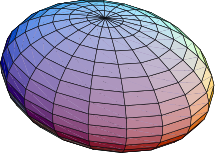
\includegraphics[width=0.2\columnwidth]{./images/ellipsoid.pdf}
		}
	\end{figure}
\end{frame}


\begin{frame}
	\frametitle{Suposiciones de Kalman Filter}
	\note{información extraida de https://youtu.be/PiCC-SxWlH8}
	
	\begin{itemize}
		\item Ruido y distribuciones Gaussianas
		\item Modelos de movimiento y observación lineales
	\end{itemize}

	\begin{align*}
		\state_{t} &= A_{t} \state_{t-1} + B_{t}\controlCommand_{t} + \motionModelNoise_{t}\\
		\observation_{t} &= C_{t} \state_{t} + \measurementModelNoise_{t}
	\end{align*}
	\note{Kalman Filter requiere que los ruidos sean gaussianos y que el estado resulte de una combinación lineal.}

	\centering
	\alert{¿qué pasa si este estas suposiciones no pasan?}
	\note{Differencial drive y Ackerman motion models NO son modelos lineales}
	\note{Los observation models de un láser  o de una cámara tampoco son lineales.}
\end{frame}

\begin{frame}
	\frametitle{Sistemas dinámicos no Non-lineales}
	\note{información extraida de https://youtu.be/PiCC-SxWlH8}
	\begin{itemize}
		\item Los problemas reales en general emplean funciones no-lineales
	\end{itemize}
	
%	\begin{align*}
%		\state_{t} &= A_{t} \state_{t-1} + B_{t}\controlCommand_{t} + \motionModelNoise_{t}\\
%		\observation_{t} &= C_{t} \state_{t} + \measurementModelNoise_{t}
%	\end{align*}

	\begin{figure}[!h]

		\includegraphics[width=0.4\columnwidth]{./images/kalman_filter_linear_equations_cross_out.pdf}
	\end{figure}

\TODO{tachar las formulas lineales}

	\begin{align*}
		\state_{t} &= \motionModelFunction{\controlCommand_{t}, \state_{t-1}} + \motionModelNoise_{t}\\
		\observation_{t} &= \observationModelFunction{\state_{t}} + \measurementModelNoise_{t}
	\end{align*}

\end{frame}


\begin{frame}
	\frametitle{Filtro de Kalman 1D}
	\note{información extraida de https://youtu.be/E-6paM_Iwfc}
	
	\begin{figure}[!h]
		\centering
		\subfloat[Predicción Inicial]
		{
			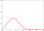
\includegraphics[width=0.3\columnwidth]{./images/kalman_filter_initial_prediction.pdf}
		}
		\subfloat[Medición]
		{
			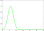
\includegraphics[width=0.3\columnwidth]{./images/kalman_filter_first_measurement.pdf}
		}
		\subfloat[Corrección]
		{
			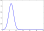
\includegraphics[width=0.3\columnwidth]{./images/kalman_filter_first_correction.pdf}
		}
	\end{figure}
	
\end{frame}

\begin{frame}
	\frametitle{Filtro de Kalman 1D}
	\note{información extraida de https://youtu.be/E-6paM_Iwfc}
	
	\begin{figure}[!h]
		\centering
		\subfloat[Predicción por Movimiento]
		{
			
\includegraphics[width=0.3\columnwidth]{./images/kalman_filter_motion_prediction.pdf}
		}
		\subfloat[Segunda Medición]
		{
			
\includegraphics[width=0.3\columnwidth]{./images/kalman_filter_second_measurement.pdf}
		}
		\subfloat[Segunda Corrección]
		{
			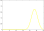
\includegraphics[width=0.3\columnwidth]{./images/kalman_filter_second_correction.pdf}
		}
	\end{figure}
	
\end{frame}


\begin{frame}
	\frametitle{Linearización en EKF: Expansión de Taylor de primer orden}
	
	\TODO{Agregar slides \url{https://www.youtube.com/watch?v=E-6paM\_Iwfc\&t=3260s}}
\end{frame}


\begin{frame}
	\frametitle{Suposición de Linealidad}
	
	\begin{figure}[!h]
		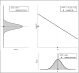
\includegraphics[width=0.5\columnwidth]{./images/linear_transformation_of_a_gaussian.pdf}
	\end{figure}
\end{frame}

\begin{frame}
	\frametitle{Función No-Lineal}
	
	\begin{figure}[!h]
		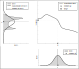
\includegraphics[width=0.5\columnwidth]{./images/nonlinear_transformation_of_a_gaussian.pdf}
	\end{figure}
\end{frame}

\begin{frame}
	\frametitle{Linearización en EKF}
	
	\begin{figure}[!h]
		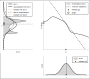
\includegraphics[width=0.5\columnwidth]{./images/linearization_applied_by_ekf.pdf}
	\end{figure}
\end{frame}


\begin{frame}
	\frametitle{Calidad de la Linearización en EKF}
	
	\begin{figure}[!h]
		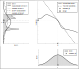
\includegraphics[width=0.5\columnwidth]{./images/dependency_approximation_quality_spread.pdf}
	\end{figure}
\end{frame}

\begin{frame}
	\frametitle{Calidad de la Linearización en EKF}
	
	\begin{figure}[!h]
		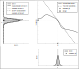
\includegraphics[width=0.5\columnwidth]{./images/dependency_approximation_quality_narrow.pdf}
	\end{figure}
\end{frame}


\begin{frame}
	\frametitle{Modelo de movimiento linearizado}
	\note{información extraida de https://youtu.be/PiCC-SxWlH8}
	
	\begin{itemize}
		\item Linearizar el modelo esta dado por:
	\begin{align*}
		p(\state_{t} | \controlCommand_{t}, \state_{t-1}) &\approx \det(2 \pi \motionParametersCovariance_{t})^{\frac{1}{2}}\\
		&\exp (-\dfrac{1}{2} (\state_{t} - \motionModelFunction{\controlCommand_{t}-\mu_{t-1}} - \motionModelJacobian_{t}(\state_{t-1}-\mu_{t-1}))^{\top}\\
		&\inverse{\motionParametersCovariance_{t}} (\state_{t} - \underbrace{\motionModelFunction{\controlCommand_{t},\mu_{t-1}} - \motionModelJacobian_{t} (\state_{t-1}-\mu_{t-1})}_{\text{modelo linearizado}}))
	\end{align*}
	
	\item $\motionParametersCovariance_{t}$ describe el ruido del movimiento
	\end{itemize}	
\end{frame}

\begin{frame}
	\frametitle{Modelo de observación linearizado}
	\note{información extraida de https://youtu.be/PiCC-SxWlH8}
	
	\begin{itemize}
		\item Linearizar el modelo esta dado por:
		\begin{align*}
			p(\observation_{t} | \state_{t}) &\approx \det(2 \pi \observationModelCovariance_{t})^{\frac{1}{2}}\\
			&\exp (-\dfrac{1}{2} (\observation_{t} - \observationModelFunction{\overline{\mu_{t}}} - \observationModelJacobian_{t}(\state_{t} - \overline{\mu_{t}}))^{\top}\\
			&\inverse{\observationModelCovariance_{t}} (\observation_{t} - \underbrace{\observationModelFunction{\overline{\mu_{t}}} - \observationModelJacobian_{t} (\state_{t}-\overline{\mu_{t}})}_{\text{modelo linearizado}}))
		\end{align*}
		
		\item $\observationModelCovariance_{t}$ describe el ruido de la medición
	\end{itemize}	
	
	
\end{frame}

\begin{frame}
	\frametitle{Algoritmo de Filtro de Kalman Extendido}
	\note{información extraída de https://youtu.be/PiCC-SxWlH8}
	
    \begin{algorithmic}[1]
    \Procedure{ExtendedKalmanFilter}{$\mu_{t-1}, \covariance_{t-1}, \controlCommand_{t}, \observation_{t}$}
        \State $\overline{\mu}_{t} = \motionModelFunction{\controlCommand_{t}, \mu_{t-1}}$
        \State $\overline{\covariance}_{t} = \motionModelJacobian_{t} \covariance_{t-1} \motionModelJacobian_{t}^{\top}+\motionParametersCovariance_{t}$
        \Statex
        \State $\kalmanGain_{t} = \overline{\covariance}_{t} \observationModelJacobian_{t}^{\top} (\observationModelJacobian_{t} \overline{\covariance}_{t}  \observationModelJacobian_{t} + \observationModelCovariance_{t})^{-1} $
        \State $\mu_{t} = \overline{\mu}_{t} + \kalmanGain_{t} (\observation_{t} - \observationModelFunction{\overline{\mu}_{t}})$
        \State $\covariance_{t} =  (I - \kalmanGain_{t} \observationModelJacobian_{t}) \overline{\covariance}_{t}$
        \State \Return $\mu_{t}, \covariance_{t}$
    \EndProcedure
    \end{algorithmic}
\end{frame}

\section{EKF Localización for feature-based map}

\begin{frame}
	\frametitle{Odometry as controls}
	\note{información extraida de https://youtu.be/PiCC-SxWlH8}
	
   	\begin{figure}[!h]
        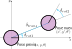
\includegraphics[width=0.6\columnwidth]{./images/odometry_as_controls.pdf}
    \end{figure}

    \begin{equation*}
        \controlCommand = (\delta_{rot1}, \delta_{trans}, \delta_{rot2})
    \end{equation*}
	
\end{frame}

\begin{frame}
	\frametitle{Motion model}
	\note{información extraida de https://youtu.be/PiCC-SxWlH8}
	
	\begin{itemize}
		\item Odometría de modelo de movimiento
		\begin{equation*}
			\begin{bmatrix}
				x^{\prime} \\
				y^{\prime} \\
				\theta^{\prime}
			\end{bmatrix} =
			\underbrace{
				\begin{bmatrix}
				x \\
				y \\
				\theta
			\end{bmatrix} +
			\begin{bmatrix}
				\delta_{trans}\cos(\theta+\delta_{rot_{1}}) \\
				\delta_{trans}\cos(\theta+\delta_{rot_{1}}) \\
				\delta_{rot_{1}} + \delta_{rot_{2}}
			\end{bmatrix}
			}_{\motionModelFunction{\controlCommand_{t}, \state_{t-1}}} + \normalDistribution{0}{\motionParametersCovariance_{t}}
		\end{equation*}
		\item Linearización
		\begin{equation*}
			\motionModelFunction{\controlCommand_{t}, \state_{t-1}} \approx 			\motionModelFunction{\controlCommand_{t}, \mu_{t-1}} + \motionModelJacobian_{t}(\state_{t-1}-\mu_{t-1})
		\end{equation*}
	\end{itemize}
	
\end{frame}

\begin{frame}
	\frametitle{Jacobianos del modelo de movimiento}
	\note{información extraida de https://youtu.be/PiCC-SxWlH8}
	Calculamos el Jacobiano con respecto al estado
	\begin{equation*}
		\motionModelJacobian_{t} = \dfrac{\delta\motionModelFunction{\controlCommand_{t},\mu_{t-1}}}{\delta \state_{t-1}} =
		\begin{bmatrix}
			\dfrac{\delta x^{\prime}}{\delta \mu_{t-1,x}} & \dfrac{\delta x^{\prime}}{\delta \mu_{t-1,y}} & \dfrac{\delta x^{\prime}}{\delta \mu_{t-1,\theta}}\\
			\dfrac{\delta y^{\prime}}{\delta \mu_{t-1,x}} & \dfrac{\delta y^{\prime}}{\delta \mu_{t-1,y}} & \dfrac{\delta y^{\prime}}{\delta \mu_{t-1,\theta}}\\
			\dfrac{\delta \theta^{\prime}}{\delta \mu_{t-1,x}} & \dfrac{\delta \theta^{\prime}}{\delta \mu_{t-1,y}} & \dfrac{\delta \theta^{\prime}}{\delta \mu_{t-1,\theta}}\\
		\end{bmatrix}
	\end{equation*}

	\begin{equation*}
	\motionModelJacobian_{t} = 
	\begin{bmatrix}
		1 & 0 & -\delta_{trans} \sin(\theta + \delta_{rot_{1}})\\
		0 & 1 & \delta_{trans} \cos(\theta + \delta_{rot_{1}})\\
		0 & 0 & 1\\
	\end{bmatrix}
	\end{equation*}
\end{frame}

\begin{frame}
	\frametitle{Jacobianos del modelo de movimiento}
	\note{información extraida de https://youtu.be/PiCC-SxWlH8}
	Calculamos el Jacobiano con respecto al comando de control
	\begin{equation*}
		\motionModelJacobianControl{t} = \dfrac{\delta\motionModelFunction{\controlCommand_{t},\mu_{t-1}}}{\delta \controlCommand_{t}} =
		\begin{bmatrix}
			\dfrac{\delta x^{\prime}}{\delta \controlCommand_{t,\delta_{rot_{1}}}} & \dfrac{\delta x^{\prime}}{\delta \controlCommand_{t,\delta_{trans}}} & \dfrac{\delta x^{\prime}}{\delta \controlCommand_{t,\delta_{rot_{2}}}}\\
			\dfrac{\delta y^{\prime}}{\delta \controlCommand_{t,\delta_{rot_{1}}}} & \dfrac{\delta y^{\prime}}{\delta \controlCommand_{t,\delta_{trans}}} & \dfrac{\delta y^{\prime}}{\delta \controlCommand_{t,\delta_{rot_{2}}}}\\
			\dfrac{\delta \theta^{\prime}}{\delta \controlCommand_{t,\delta_{rot_{1}}}} & \dfrac{\delta \theta^{\prime}}{\delta \controlCommand_{t,\delta_{trans}}} & \dfrac{\delta \theta^{\prime}}{\delta \controlCommand_{t,\delta_{rot_{2}}}}
		\end{bmatrix}
	\end{equation*}
	
	\begin{equation*}
		\motionModelJacobianControl_{t} = 
		\begin{bmatrix}
			-\delta_{trans} \sin(\theta + \delta_{rot_{1}}) & \cos(\theta + \delta_{rot_{1}}) & 0\\
			\delta_{trans} \cos(\theta + \delta_{rot_{1}}) & \sin(\theta + \delta_{rot_{1}}) & 0\\
			0 & 0 & 1\\
		\end{bmatrix}
	\end{equation*}
\end{frame}

\begin{frame}
	\frametitle{Modelo de observación}
	\note{información extraida de https://youtu.be/PiCC-SxWlH8}
	\begin{itemize}
	\item Modelo de distancia y orientación (range-bearing model)
	\begin{equation*}
		\observation_{t}^{i} =
		\begin{bmatrix}
			r_{t}^{i}\\
			\phi_{t}^{i} 
		\end{bmatrix} =
		\begin{bmatrix}
			\sqrt{(m_{j,x}-x)^{2} + (m_{j,y}-y)^{2}}\\
			\atantwo(m_{j,y}-y, m_{j,x}-x) -\theta
		\end{bmatrix}
		+ \normalDistribution{0}{\observationModelCovariance_{t}}		
	\end{equation*}
	
	\item Linearización
	\begin{equation*}
	\observationModelFunction{\state_{t}, m} \approx 			\observationModelFunction{\overline{\mu}_{t}} + \observationModelJacobian_{t}^{i}(\state_{t}-\overline{\mu}_{t})
	\end{equation*}
	\end{itemize}
	
\end{frame}

\begin{frame}
	\frametitle{Jacobianos del modelo de observación}
	\note{información extraida de https://youtu.be/PiCC-SxWlH8}
	Calculamos el Jacobiano con respecto al estado
	\begin{equation*}
		\observationModelJacobian_{t} = \dfrac{\delta\observationModelFunction{\overline{\mu}_{t},m}}{\delta \state_{t-1}} =
		\begin{bmatrix}
			\dfrac{\delta r_{t}^{i}}{\delta \overline{\mu}_{t,x}} & \dfrac{\delta r_{t}^{i}}{\delta \overline{\mu}_{t,y}} & \dfrac{\delta r_{t}^{i}}{\delta \overline{\mu}_{t,\theta}}\\
			\dfrac{\delta \phi_{t}^{i}}{\delta \overline{\mu}_{t,x}} & \dfrac{\delta \phi_{t}^{i}}{\delta \overline{\mu}_{t,y}} & \dfrac{\delta \phi_{t}^{i}}{\delta \overline{\mu}_{t,\theta}}
		\end{bmatrix}
	\end{equation*}
	
	\begin{equation*}
		\observationModelJacobian_{t}^{i} = 
		\begin{bmatrix}
			-\dfrac{m_{j,x} - \overline{\mu}_{t,x}}{\sqrt{q}} & -\dfrac{m_{j,y} - \overline{\mu}_{t,y}}{\sqrt{q}}  & 0\\
			-\dfrac{m_{j,y} - \overline{\mu}_{t,y}}{q}  & -\dfrac{m_{j,x} - \overline{\mu}_{t,x}}{q}  & -1
		\end{bmatrix}
	\end{equation*}
	donde
	\begin{equation*}
		q = (m_{j,x}-\overline{\mu}_{t,x})^{2} + (m_{j,y}-\overline{\mu}_{t,y})^{2}
	\end{equation*}
\end{frame}

\begin{frame}
	\frametitle{Algoritmo de Filtro de Kalman Extendido}
	\note{información extraida de https://youtu.be/PiCC-SxWlH8}
	
 	\begin{algorithmic}[1]
		\State ExtendedKalmanFilter({$\mu_{t-1}, \covariance_{t-1}, \controlCommand_{t}, \observation_{t}$, $c_{t}$, $m$})
		\State $\theta = \mu_{t-1,\theta}$
		
		\State $
			\motionModelJacobian_{t} = 
			\begin{bmatrix}
				1 & 0 & -\delta_{trans} \sin(\theta + \delta_{rot_{1}})\\
				0 & 1 & \delta_{trans} \cos(\theta + \delta_{rot_{1}})\\
				0 & 0 & 1\\
			\end{bmatrix}
			   $
		\State $
			\motionModelJacobianControl_{t} = 
			\begin{bmatrix}
				-\delta_{trans} \sin(\theta + \delta_{rot_{1}}) & \cos(\theta + \delta_{rot_{1}}) & 0\\
				\delta_{trans} \cos(\theta + \delta_{rot_{1}}) & \sin(\theta + \delta_{rot_{1}}) & 0\\
				0 & 0 & 1\\
			\end{bmatrix}
         	   $
		\State $
			\motionModelCovariance_{t} = 
			\begin{bmatrix}
				\alpha_{1}\delta^{2}_{rot_{1}} + \alpha_{2}\delta^{2}_{trans} & 0 & 0\\
				0 & \alpha_{3} \delta^{2}_{trans} + \alpha_{4} \left( \delta^{2}_{rot_{1}} + \delta^{2}_{rot_{2}} \right) & 0\\
				0 & 0 & \alpha_{1}\delta^{2}_{rot_{1}} + \alpha_{2}\delta^{2}_{trans}\\
			\end{bmatrix}
			  $
		\State $\overline{\mu}_{t} = \mu_{t-1} + 
			\begin{bmatrix}
			\delta_{trans}\cos(\theta+\delta_{rot_{1}}) \\
			\delta_{trans}\cos(\theta+\delta_{rot_{1}}) \\
			\delta_{rot_{1}} + \delta_{rot_{2}}
		\end{bmatrix}$
		\State $\overline{\covariance}_{t} = \motionModelJacobian_{t} \covariance_{t-1} \motionModelJacobian_{t}^{\top}+\motionModelJacobianControl_{t} \motionModelCovariance_{t} \motionModelJacobianControl_{t}^{\top}$
	\end{algorithmic}
	
\end{frame}

\begin{frame}
	\frametitle{Prediction step}
	\note{información extraida de https://youtu.be/PiCC-SxWlH8}
	
	\begin{figure}[!h]
		\includegraphics[width=0.5\columnwidth]{./images/prediction_step.pdf}
	\end{figure}
	
\end{frame}

\begin{frame}
	\frametitle{Algoritmo de Filtro de Kalman Extendido}
	\note{información extraida de https://youtu.be/PiCC-SxWlH8}
	\footnotesize
 	\begin{algorithmic}[1]
		\State
		$ \observationModelCovariance_{t} =
			\begin{bmatrix}
				\sigma_{r}^{2} & 0\\
				0 & \sigma_{\phi}^{2}
			\end{bmatrix}
		$
		\For todos los features observados $z_{t}^{i} = (r_{t}^{i}, \phi_{t}^{i})^{\top}$
		
		\State $ j = c_{t}^{i}$
		\State $ q = (m_{j,x}-\overline{\mu}_{t,x})^{2} + (m_{j,y}-\overline{\mu}_{t,y})^{2} $
		\State
		$ \hat{\observation}_{t}^{i} =
			\begin{bmatrix}
				\sqrt{q}\\
				\atantwo(m_{j,y}-\overline{\mu}_{t,y}, m_{j,x}-\overline{\mu}_{t,x}) - \overline{\mu}_{t,\theta}
			\end{bmatrix}
		$
		\State
		$ \observationModelJacobian_{t}^{i} = 
			\begin{bmatrix}
				-\dfrac{m_{j,x} - \overline{\mu}_{t,x}}{\sqrt{q}} & -\dfrac{m_{j,y} - \overline{\mu}_{t,y}}{\sqrt{q}}  & 0\\
				-\dfrac{m_{j,y} - \overline{\mu}_{t,y}}{q}  & -\dfrac{m_{j,x} - \overline{\mu}_{t,x}}{q}  & -1
			\end{bmatrix}
		$
		
		\State $S_{t}^{i} = \observationModelJacobian_{t}^{i} \overline{\covariance}_{t} \observationModelJacobian_{t}^{i^{\top}} + \observationModelCovariance_{t} $

		\State $\kalmanGain_{t}^{i} = \overline{\covariance}_{t} {\observationModelJacobian_{t}^{i}} \overline{\covariance}_{t} \observationModelJacobian_{t}^{i^{\top}} S_{t}^{i^{-1}} $
		\State $\overline{\mu}_{t} = \overline{\mu}_{t} + \kalmanGain_{t}^{i}(\observation_{t} - \hat{\observation}_{t}^{i})$
		\State $\overline{\covariance}_{t} = (I - \kalmanGain_{t}^{i}\observationModelJacobian_{t}^{i})\overline{\covariance}_{t}$
		
		\EndFor
		\State $\mu_{t} = \overline{\mu}_{t}$
		\State $\covariance_{t} = \overline{\covariance}_{t}$
		
		\State \Return $\mu_{t}, \covariance_{t}$
	\end{algorithmic}
	
	
\end{frame}

\begin{frame}
	\frametitle{Medición esperada}
	\note{información extraida de https://youtu.be/PiCC-SxWlH8}
	
	\begin{figure}[!h]
		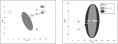
\includegraphics[width=\columnwidth]{./images/measurement_prediction.pdf}
	\end{figure}
	
\end{frame}

\begin{frame}
	\frametitle{Correction step}
	\note{información extraida de https://youtu.be/PiCC-SxWlH8}
	
	\begin{figure}[!h]
			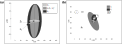
\includegraphics[width=\columnwidth]{./images/correction_step.pdf}
	\end{figure}
	
\end{frame}

\begin{frame}
	\frametitle{Ejemplo: EKF Localization 2D}
	\note{información extraida de libro Probabilistic Robotics}
	
	\begin{figure}[!h]
		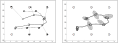
\includegraphics[width=\columnwidth]{./images/ekf_localization_example.pdf}
	\end{figure}
	
\end{frame}

\begin{frame}
	\frametitle{Resumen de EKF}
	\note{información extraida de https://youtu.be/PiCC-SxWlH8}
	
	\begin{itemize}
		\item Es una extensión del Filtro de Kalman
		\item Una forma de trabajar con no-lineridades
		\item Realiza linearizaciones locales
		\item Funciona bien en la práctica para casos moderadamente no lineales
		\item Grandes incertidumbres conllevan un incremento del error
	\end{itemize}
	
\end{frame}



   	\section{Filtro de Partículas}
    \begin{frame}
    \frametitle{Filtro de Partículas (Particle Filter)}
    \note{Información extraída de Vídeo de Cyrill Stachniss https://youtu.be/MsYlueVDLI0}
    \footnotesize
    \begin{itemize}
        \item Con EKF estamos restringidos a distribuciones Gaussianas.
        \item Cuando usamos EKF obtenemos una Distibuión Gaussiana que describe dónde se encuentra el robot.
        \item En Particle Filter utilizamos partículas o hipótesis que describen dónde podría estar el robot.
        \item En vez de tener una forma paramétrica como es EKF, que describimos la distribución de probabilidad con los parámetros media $\mu$ y covarianza $\covariance$. Partible Filter utiliza muestras no-paramétricas como hipótesis sobre dónde el robot podría estar.
    \end{itemize}
    
    
   	\begin{center}
        \movie[loop]{\includegraphics[width=0.4\columnwidth]{images/particle_filter/particle_filter_video.jpg}}{videos/particle_filter.mp4}
    \end{center}
    
    \note{Vídeo extraído de https://rse-lab.cs.washington.edu/projects/mcl/animations/global-floor.gif}
    
\end{frame}

\begin{frame}
    \frametitle{Aproximación de una Función}
    \note{Información extraída de Vídeo de Cyrill Stachniss https://youtu.be/MsYlueVDLI0}
    \footnotesize
    
    \begin{itemize}
        \item Objetivo: Poder estimar cualquier \textbf{distribución de probabilidad arbitraria}.
    \end{itemize}
    
    \begin{center}
    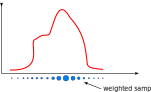
\includegraphics[width=0.5\columnwidth]{./images/particle_filter/arbitrary_distribution.pdf}
    \end{center}
    
\end{frame}

\begin{frame}
    \frametitle{Utilizando Muestras (Partículas)}
    \note{Información extraída de Vídeo de Cyrill Stachniss https://youtu.be/MsYlueVDLI0}
    \footnotesize
    \begin{itemize}
        \item \textbf{Múltiples muestras} para representar una distribución de probabilidad arbitraría
        \item Las muestras son están más agrupadas en algunas áreas en otras menos. La cantidad de partículas por unidad de área describe que tan probable es que el robot se encuentre en esa área.
        \item Cada muestra está acumulando un poco de ``masa de probabilidad''.
        \item Las muestra puede ser vista como una aproximación a la función de densidad de probabilidad (pdf).
        \item Para obtener la pdf, hay que integrar sobre una cierta área de manera de obtener la probabilidad matemática de que el robot se encuentre en dicha área.
    \end{itemize}
    
    \begin{center}
    \includegraphics[width=0.5\columnwidth]{./images/particle_filter/arbitrary_distribution_samples.pdf}
    \end{center}
    
\end{frame}

\begin{frame}
    \frametitle{Utilizando Muestras con Peso}
    \note{Información extraída de Vídeo de Cyrill Stachniss https://youtu.be/MsYlueVDLI0}
    \footnotesize
    \begin{itemize}
        \item \textbf{Múltiples muestras con peso} para representar una distribución de probabilidad arbitraría
        \item Es posible reducir el número de muestras que necesitamos, si le agregamos pesos a cada muestra
        \item Mientras más peso tiene una muestra, más masa de probabilidad hay en esa región
        \item Los pesos de todas las partículas juntas deben sumar 1
        \item Al inicio, podríamos agregarle a cada muestra un peso uniforme. Por ejemplo, si tenemos $n$ muestras, entonces cada muestra tiene peso $\frac{1}{n}$
    \end{itemize}
    
    \begin{center}
        \includegraphics[width=0.5\columnwidth]{./images/particle_filter/arbitrary_distribution_weighted_samples.pdf}
    \end{center}
    
\end{frame}

\begin{frame}
    \frametitle{Filtro de Partículas (Particle Filter)}
    \note{Información extraída de Vídeo de Cyrill Stachniss https://youtu.be/MsYlueVDLI0}
    
    \footnotesize
    \begin{itemize}
        \item Notar que es una aproximación de la pdf
        \item Es importante tener un número de muestras suficientes para poder representar la fdp adecuadamente.
    \end{itemize}
    
    
\end{frame}

\begin{frame}
    \frametitle{Conjunto de Partículas}
    
    \begin{itemize}
        \item Conjunto de partículas con peso
            
        \begin{center}
            
\includegraphics[width=0.5\columnwidth]{./images/particle_filter/weighted_samples.pdf}
        \end{center}

        \item Las partículas representan la posterior belief dada por
        \begin{equation*}
            p(x) = \sum_{j=1}^{J} w^{[j]} \delta_{x^{[j]}}(x)    
        \end{equation*}
        donde $\delta_{x^{[j]}}(x)$ es la función de Dirac centrada en la ubicación de la partícula $x^{[j]}$.

        \begin{equation*}
            \delta(y) = 
            \begin{cases} 
            \infty, & y = x^{[j]} \\ 
            0, & y \neq x^{[j]} 
            \end{cases};    
        \end{equation*}

        \note{La función tiende a infinito cuando $x=j$ y, para cualquier otro valor de $x$, es igual a 0.}

    \end{itemize}
   
\end{frame}


\begin{frame}
    \frametitle{Partículas para Aproximar}
    
    \begin{itemize}
        \item Partículas para aproximar una función
        
        \begin{center}
            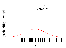
\includegraphics[width=0.45\columnwidth]{./images/particle_filter/gaussian_approximation_by_sampling.pdf}
            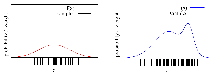
\includegraphics[width=0.45\columnwidth]{./images/particle_filter/particles_for_approximation.pdf}
        \end{center}

        \item Más partículas caen en una región, más alta es la probabilidad de la región
    \end{itemize}
    
    \begin{center}
        \alert{¿Cómo obtener dichas muestras?}
    \end{center}

\end{frame}

\begin{frame}
    \frametitle{Una Forma Cerrada de Muestreo es solo posible para Pocas Distribuciones }
    \begin{itemize}
        \item Ejemplo: Distribución Gaussiana
        
        \begin{center}
            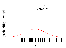
\includegraphics[width=0.5\columnwidth]{./images/particle_filter/gaussian_approximation_by_sampling.pdf}
        \end{center}
        
        \begin{equation*}
            x \leftarrow \frac{1}{2} \sum_{i=1}^{12} \text{rand}(-\sigma, \sigma)
        \end{equation*}
    \end{itemize}

    ¿Cómo samplear utilizando otra distribución?

    \note{Técnica de rejection sampling. No sé utiliza en particle filter porque es una técnica muy ineficiente.}

    \note{Técnica Importance Sampling Principle}

\end{frame}
    


\begin{frame}
    \frametitle{Principio de muestreo de importancia}
    \begin{itemize}
        \item Podemos usar una distribución diferente $\pi$ para generar muestras de $f$
        \item Considere las ``diferencias entre $\pi$ y $f$'' usando un peso $w = f(x) / \pi(x)$
        \item Target $f$
        \item Proposal $\pi$
        \item Precondición:
        $f(x) > 0 \implies \pi(x) > 0$
        \begin{center}
        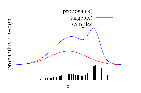
\includegraphics[width=0.45\textwidth]{./images/particle_filter/importance_sampling_principle.pdf}
        \end{center}
    \end{itemize}
\end{frame}
    
\begin{frame}
    \frametitle{Filtro de Partículas}
    \begin{itemize}
        \item Filtro Bayesiano recursivo
        \item Enfoque no paramétrico
        \item Modela la distribución mediante muestras
        \item \textbf{Predicción}: extraer de la distribución propuesta
        \item \textbf{Corrección}: ponderación por la relación entre la distribución objetivo y la propuesta
        \item \alert{¡Cuantas más muestras usemos, mejor será la estimación!}
    \end{itemize}
\end{frame}
    
\begin{frame}
    \frametitle{Algoritmo de Filtro de Partículas}
    \begin{enumerate}
        \item Muestrear las partículas utilizando la distribución propuesta.
        \begin{equation*}
            x_t^{[j]} \sim proposal(x_t | \ldots)
        \end{equation*}
        \item Calcular los pesos de importancia
        \begin{equation*}
            w_t^{[j]} = \frac{target(x_t^{[j]})}{proposal(x_t^{[j]})}
        \end{equation*}
        \item Resampling: Tomar la partícula $i$ con probabilidad $w_t^{[j]}$ y repetir $J$ veces 
    \end{enumerate}
    \note{Reemplazar muestras improbables por otras más probables}
\end{frame}

\begin{frame}
    \frametitle{Algoritmo de Filtro de Partículas}
    \begin{algorithmic}[1]
    \Procedure{ParticleFilter}{$\mathcal{X}_{t-1}, u_{t}, z_{t}$}:
    \State $\bar{\mathcal{X}}_t = \mathcal{X}_t = \emptyset$
    \For{$j = 1$ to $J$}
        \State sample $x_t^{[j]} \sim \pi(x_t)$
        \State $w_t^{[j]} = \dfrac{p(x_t^{[j]})}{\pi(x_{t}^{[j]})}$
        \State $\bar{\mathcal{X}}_t = \bar{\mathcal{X}}_t + \langle x_t^{[j]}, w_t^{[j]}\rangle$
    \EndFor
    \For{$j = 1$ to $M$}
        \State Draw $i$ with probability $\propto w_t^{[i]}$
        \State Add $x_t^{[i]}$ to $\mathcal{X}_t$
    \EndFor
    \State return $\mathcal{X}_t$
    \EndProcedure
    \end{algorithmic}
\end{frame}


\begin{frame}
    \frametitle{Monte Carlo Localization}

    Monte Carlo Localization: Filtro de Partículas para la localización de un robot

\end{frame}


% \begin{frame}
%     \frametitle{Monte Carlo Localization}

%     \begin{center}
%         \includegraphics[width=0.37\textwidth]{./images/particle_filter/monte_carlo_localization_example.pdf}
%     \end{center}

% \end{frame}

\begin{frame}
    \frametitle{Monte Carlo Localization}
    \begin{itemize}
        \item Cada partícula es una hipótesis de la pose
        \item Proposal es el motion model
        \begin{equation*}
            x_t^{[j]} \sim p(x_t \, | \, x_{t-1}, u_t)
        \end{equation*}
        \item Corrección vía el observation model
        \begin{equation*}
            w_t^{[j]} = \frac{target}{proposal} \propto p(z_t \, | \, x_t, m)
        \end{equation*}
    \end{itemize}
\end{frame}

    
\begin{frame}
    \frametitle{Filtro de Partículas para Localización}
    \begin{algorithmic}[1]
        \Procedure{ParticleFilter}{$\mathcal{X}_{t-1}, u_{t}, z_{t}$}
        \State $\bar{\mathcal{X}}_t = \mathcal{X}_t = \emptyset$
        \For{$j = 1$ to $J$}
            \State Sample $x_t^{[j]} \sim p(x_t \, | \, u_t, x_{t-1}^{[j]})$
            \State $w_t^{[j]} = p(z_t \, | \, x_t^{[j]})$
            \State $\bar{\mathcal{X}}_t = \bar{\mathcal{X}}_t + \langle x_t^{[j]}, w_t^{[j]}\rangle$
        \EndFor
        \For{$i = 1$ to $J$}
            \State Draw $i \in 1,\ldots,J$ with probability $\propto w_t^{[i]}$
            \State Add $x_t^{[i]}$ to $\mathcal{X}_t$
        \EndFor
        \State return $\mathcal{X}_t$
    \EndProcedure
    \end{algorithmic}
\end{frame}
    
\begin{frame}
    \frametitle{Monte Carlo Localization - Paso de Corrección}

    \begin{center}
        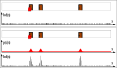
\includegraphics[width=0.8\textwidth]{./images/particle_filter/monte_carlo_correction.pdf}
    \end{center}

\end{frame}

\begin{frame}
    \frametitle{Monte Carlo Localization - Remuestreo y Predicción}

    \begin{center}
        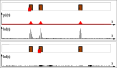
\includegraphics[width=0.8\textwidth]{./images/particle_filter/monte_carlo_resample_and_predict.pdf}
    \end{center}

\end{frame}

\begin{frame}
    \frametitle{Monte Carlo Localization - Paso de Corrección 2}

    \begin{center}
        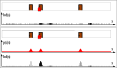
\includegraphics[width=0.8\textwidth]{./images/particle_filter/monte_carlo_correction2.pdf}
    \end{center}

\end{frame}

\begin{frame}
    \frametitle{Monte Carlo Localization - Remuestreo y Predicción 2}

    \begin{center}
        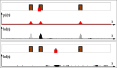
\includegraphics[width=0.8\textwidth]{./images/particle_filter/monte_carlo_resample_and_predict2.pdf}
    \end{center}

\end{frame}


\begin{frame}
    \frametitle{Resampling}
    \begin{itemize}
        \item Tomar la partícula $i$ con probabilidad $w_t^{[i]}$. Repetir $J$ veces.
        \item Informalmente: ``Reemplazar muestras improbables por otras más probables''
        \item Supervivencia del más apto
        \item ``Truco'' para evitar que muchas muestras cubran estados improbables
        \item Necesario, ya que tenemos un número limitado de muestras
    \end{itemize}
\end{frame}
    
\begin{frame}
    \frametitle{Métodos de Resampling}
    \begin{overlayarea}{\textwidth}{\textheight}
        
        \only<1>{
            \begin{center}
                \includegraphics[width=0.35\textwidth]{./images/particle_filter/resampling_rulette_wheel1.pdf}
            \end{center}
        }
        \only<2>{
            \begin{center}
                \includegraphics[width=0.35\textwidth]{./images/particle_filter/resampling_rulette_wheel2.pdf}
            \end{center}
        }
        \only<3>{
            \begin{center}
                \includegraphics[width=0.35\textwidth]{./images/particle_filter/resampling_rulette_wheel3.pdf}
            \end{center}
        }
        \only<3>{
            \begin{itemize}
                \item Roulette Wheel
                \item Búsqueda binaria para saber en qué bucket cae la bola ($O(J \log(J))$)
            \end{itemize}
            \note{Los buckets de la ruleta representan los pesos de las partículas. Mientras más grande el bucket, más probable es que esta partícula sea seleccionada.}
            \note{Tenemos que hacerlo J veces. Tenemos que encontrar dónde cae la bola. Esto lo podemos hacer con binary-search. La suma de todos los pesos de la ruleta es 1. Si tiramos un número random entre 0 y 1 entonces con búsqueda binaria podemos saber en qué bucket cae.}
        }
    \end{overlayarea}
\end{frame}

\begin{frame}
    \frametitle{Métodos de Resampling}
    \begin{overlayarea}{\textwidth}{\textheight}
        \only<1>{
            \begin{center}
                \includegraphics[width=0.35\textwidth]{./images/particle_filter/resampling_stochastic_universal_sampling1.pdf}
            \end{center}
        }
        \only<2>{
            \begin{center}
                \includegraphics[width=0.35\textwidth]{./images/particle_filter/resampling_stochastic_universal_sampling2.pdf}
            \end{center}
        }

        \only<2>{

        \begin{itemize}
            \item Stochastic universal sampling (utilizando $J$ flechas equidistantes)
            \item También llamado \emph{Low-Variance Resampling} (evita que las partículas se concentren rápidamente)
            \item $O(J)$
        \end{itemize}
        \note{Utilizando on flechas y poniendolas equidistantes. Rotamos todas juntas y elejimos de a n partículas. Por tanto cuando, tiro un número random ahora se seleccionan las J partículas de una.}
        \note{Tiene costo computacional lineal porque solo tengo que recorrer los pesos una vez para ver dónde caen todas las flechas.}
        \note{Ejemplo 8 flechas distante 45 grados una de otra.}
        
        }
    \end{overlayarea}
\end{frame}

\begin{frame}
    \frametitle{Resampling}
    \begin{itemize}
        \item Muestreo con remplazo (muestreamos tomando una partícula y luego la volvemos a colocar en la bolsa)
        \item Roulette Wheel resampling es fácil de entender pero es suboptimo en la práctica
        \item \alert{¿Qué pasa si todas las partículas tienen el mismo peso?}
        \note{Si todas las partículas tienen el mismo peso, sería como tener un sensor que no me da información.}
        \note{Si todas las partículas tienen el mismo peso, el resampling seleccionará partículas de manera aleatoria y las duplicará, y otras partículas no serán seleccionadas y moriran. Y esto pasa sin que una partícula sea mejor que otra. Esto lleva a que el sistema converja en una localización cualquiera.}
        \note{Por tanto, si todas las partículas tienen el mismo peso entonces no tiene sentido escoger una por encima de otra.}

        \note{
            https://robotics.stackexchange.com/questions/16093/why-does-the-low-variance-resampling-algorithm-for-particle-filters-work

            TLDR; A particle filter’s convergence rate is inversely proportional to the variance in the parents’ offspring counts. Low variance means fast convergence.

            NOTE: Below, I discuss (but never explicitly mention) the concept of variance effective population size.

            The effectiveness of this resampling strategy makes a lot of sense when you consider that the particle filter is, at its core, an evolutionary algorithm (EA). All EAs tend to lose diversity because of the random sampling step, at a rate proportional to the variance in how many offspring the parents produce. This effect is known as genetic drift, and it adversely affects biological populations as well. As a result of this diversity loss, the EA prematurely converges to suboptimal solutions. This is bad news.

            Intuitively, genetic drift makes sense. When parents are chosen at random (the most common setup), those with low fitness/quality are likely to get skipped and produce zero offspring and be eliminated from the gene pool, thus reducing the population’s diversity. Now, the rate at which natural selection improves a population’s fitness is directly proportional to the population’s diversity—diversity is literally the fuel that drives natural selection. Genetic drift reduces the the diversity, thus decreasing the rate at which the population’s fitness can improve and causing the aforementioned bad news.

            Let’s now look at the low-variance resampling method. This method gives almost every parent exactly the number of offspring that they would be expected to get with the random sampling, without the extra uncertainty (variance). This reduces genetic drift and greatly increases the efficiency with which the particle filter can improve its solution and/or adapt to changing condition
        }

    \end{itemize}
\end{frame}

    
\begin{frame}
    \frametitle{Low Variance Resampling}
    \begin{algorithmic}[1]
    \Procedure{Low Variance Resampling}{$\mathcal{X}_{t}$,$\mathcal{W}_{t}$}
    \State $\bar{\mathcal{X}}_t = \emptyset$
    \State $r = \text{rand}(0; J^{-1})$
    \State $c = w_t^{[1]}$
    \State $i = 1$
    \For{$j = 1$ to $J$}
        \State $U = r + (j - 1)  J^{-1}$
        \While{$U > c$}
            \State $i = i + 1$
            \State $c = c + w_t^{[i]}$
        \EndWhile
        \State Add $x_t^{[i]}$ to $\bar{\mathcal{X}}_t$
    \EndFor
    \State Return $\bar{\mathcal{X}}_t$
    \EndProcedure
    \end{algorithmic}
\end{frame}

\begin{frame}
    \frametitle{Low Variance Resampling}
    \begin{itemize}
        \item Realiza un remuestreo que mantiene las muestras en el caso que tengan pesos iguales
        \item Es más rápido que el remuestreo con roulette wheel: $\mathcal{O}(J)$ vs. $\mathcal{O}(J \log J)$
        \item \alert{Utilizaremos siempre Low Variance Resampling!}
    \end{itemize}
\end{frame}


\begin{frame}
    \frametitle{Desventajas}
    \begin{itemize}
        \item No escala bien para espacios de alta dimensionalidad
        \item Problemático en situaciones con mucha incertidumbre
        \item Problema agotamiento de partículas
    \end{itemize}
\end{frame}

\begin{frame}
    \frametitle{Ventajas}
    \begin{itemize}
        \item Puede trabajar con distribuciones no Gaussianas
        \item Funciona bien en espacios de baja dimensionalidad
        \item Puede manejar ambiguedades en la asociación de los datos
        \item Puede incorporar fácilmente diferentes modalidades de sensado
        \item Robusto
        \item Fácil de implementar
    \end{itemize}
\end{frame}

\begin{frame}
    \frametitle{Resumen – Particle Filter}
    \begin{itemize}
        \item Los filtros de partículas son filtros bayesianos recursivos y no paramétricos
        \item El Posterior Belief se representa mediante un conjunto de muestras ponderadas
        \item No se limita a Distribuciones Gaussianas
        \item Proposal para extraer muestras en $t+1$
        \item Peso para tener en cuenta las diferencias entre la proposal y el target
    \end{itemize}
\end{frame}
    
\begin{frame}
    \frametitle{Resumen – Localización con PF}
    \begin{itemize}
        \item Las partículas se propagan según el modelo de movimiento
        \item Se ponderan según la probabilidad de la observación
        \item Se denomina Localización de Monte Carlo (MCL)
        \item La MCL es un gold standard para la localización de robots móviles en entornos \emph{indoor}
    \end{itemize}
\end{frame}



\begin{frame}
    \frametitle{Material para Particle Filter}
    
    \begin{itemize}
        \item Información extraída de Vídeo de Cyrill Stachniss https://youtu.be/MsYlueVDLI0
        \item https://rse-lab.cs.washington.edu/projects/mcl/
        \item http://ais.informatik.uni-freiburg.de/teaching/ws12/mapping/pdf/slam09-particle-filter.pdf
    \end{itemize}
   
\end{frame}


\begin{frame}
    \frametitle{TODO}
    \note{Información extraída de Vídeo de Cyrill Stachniss https://youtu.be/MsYlueVDLI0}
    \note{https://rse-lab.cs.washington.edu/projects/mcl/}
    
    \TODO{UTILIZAR LAS SLIDES DEL SEMINARIO}
    
    
\end{frame}


    

	
	\section{Bibliografía}
	\section{Bibliografía}
\begin{frame}
    \frametitle{Bibliografía}
    \nocite{siegwart2011introduction}
    \nocite{corke2017robotics}
    \nocite{hartley2003multiple}
    \nocite{misra2006global}

    \printbibliography

\end{frame}
	
	% Programming a robotic car seminar slides
	%\section{Medición}

\begin{frame}{Belief luego de sensar}
	\begin{block}{Ejemplo}
		\begin{itemize}
			\item Un mundo constituido por cinco celdas $x_{i}$ donde $i = 1, \dots ,5$
			\item Las celdas $x_{2}$ y $x_{3}$ son rojas, y el resto verdes.
			\item Inicialmente el robot desconoce su posición
			\item La probabilidad de que el robot sense correctamente  esta dada por la siguiente distribución de probabilidades:
			
			\begin{displaymath}
				P(sensa \ color | x_{i} = color) = 0.6
			\end{displaymath}
			\begin{displaymath}
				P(sensa \ \neg color | x_{i} = color) = 0.2
			\end{displaymath}
			
			Observar que no es una distribución de probabilidad correcta ya que la suma debe ser $1$.
			
		\end{itemize}
		
	\end{block}
	
	\begin{center}
		\includegraphics<1>[height=1.0cm]{./images/uniform_five_cells.png}
	\end{center}
	
\end{frame}

\begin{frame}{Belief luego de sensar}
	
	Si el robot \alert{sensa rojo}, ?`Cuál es su Posterior belief?
	
	\begin{center}
		\includegraphics<1>[height=3.5cm]{./images/inaccurate_sensing_quiz.png}
	\end{center}
\end{frame}

\begin{frame}{Belief luego de sensar}
	
	Si el robot \alert{sensa rojo}, ?`Cuál es su Posterior belief?
	
	\begin{center}
		\includegraphics<1>[height=3.5cm]{./images/inaccurate_sensing_solution.png}
	\end{center}
	\begin{footnotesize}
		\begin{displaymath}
			P(x_{i} = rojo | sensa \ rojo) = P(sensa \ rojo | x_{i} = rojo) P(x_{i}) = 0.2 \times 0.6 = 0.12
		\end{displaymath}
		\begin{displaymath}
			P(x_{i} = verde | sensa \ rojo) = P(sensa \ rojo | x_{i} = verde) P(x_{i}) = 0.2 \times 0.2 = 0.04
		\end{displaymath}
	\end{footnotesize}
	
\end{frame}

\begin{frame}{Belief luego de sensar}
	\begin{displaymath}
		P(x_{i} = rojo | sensa \ rojo) = 0.12
	\end{displaymath}
	\begin{displaymath}
		P(x_{i} = verde | sensa \ rojo) = 0.04
	\end{displaymath}
	
	Observar que estamos ante una distribución de probabilidades formalmente incorrecta dado que la suma: 
	\begin{displaymath}
		\sum_{i=1}^{5} P(x_{i}) = 0.04 + 0.12 + 0.12 + 0.04 + 0.04 = 0.36
	\end{displaymath}
	
	
	Si normalizamos la distribución, queda:
	
	\begin{displaymath}
		P(x_{i} = rojo| sensa \ rojo) = \dfrac{0.12}{0.36} = \dfrac{1}{3}
	\end{displaymath}
	\begin{displaymath}
		P(x_{i} = verde| sensa \ rojo) = \dfrac{0.04}{0.36} = \dfrac{1}{9}
	\end{displaymath}
	
	En general, $P(x_{i}|z)$ es la distribución Posterior belief del lugar $x_{i}$ dada la medición $z$.
\end{frame}


\begin{frame}{Regla de Bayes}
	
	Notar que cuando el robot sensa no hace otra cosa que aplicar la Regla Bayes:
	
	\begin{block}{Regla de Bayes}
		\begin{displaymath}
			P(x_{i} | z) = \dfrac{P(z | x_{i})P(x_{i})} {P(z)} 
		\end{displaymath}
		$P(x_{i} | z)$ : probabilidad a Posteriori (Posterior Belief) \\
		$P(z | x_{i})$ : probabilidad de Medición \\
		$P(x_{i})$ : probabilidad a Priori \\
		$P(z)$ : término de Normalización
	\end{block}
	
\end{frame}

\section{Motricidad}
\begin{frame}{Belief luego del movimiento}
	\begin{block}{Ejemplo (continuación)}
		\begin{itemize}
			\item Un mundo \alert{cíclico} constituido por cinco celdas $x_{i}$ donde $i = 1, \dots ,5$
			\item La distribución de probabilidad a priori esta determinada por:
			\begin{displaymath}
				P(x_{1}) = P(x_{4}) = P(x_{5}) = \dfrac{1}{9}
			\end{displaymath}
			\begin{displaymath}
				P(x_{2}) = P(x_{3}) = \dfrac{1}{3}	
			\end{displaymath}
		\end{itemize}
	\end{block}
	
\end{frame}

\begin{frame}{Belief luego del movimiento}
	Si el robot tiene una \alert{motricidad exacta} y desea moverse \alert{una} celda a la derecha, ?`Cuál es su Posterior belief?
	
	\begin{center}
		\includegraphics<1>[height=3.5cm]{./images/exact_motion_quiz.png}
	\end{center}
	
\end{frame}

\begin{frame}{Belief luego del movimiento}
	Si el robot tiene una \alert{motricidad exacta} y desea moverse \alert{una} celda a la derecha, ?`Cuál es su Posterior belief?
	
	\begin{center}
		\includegraphics<1>[height=3.5cm]{./images/exact_motion_solution.png}
	\end{center}
	
\end{frame}

\begin{frame}{Belief luego del movimiento}
	Suponiendo ahora que el robot desea moverse \alert{dos} celdas a la derecha y tiene una \alert{motricidad inexacta} con la siguiente distribución de probabilidad:
	\begin{columns}[t]
		\begin{column}{5cm}
			\begin{displaymath}
				P(x_{i+2}| x_{i}) = 0.8
			\end{displaymath}
			\begin{displaymath}
				P(x_{i+1}| x_{i}) = 0.1
			\end{displaymath}
			\begin{displaymath}
				P(x_{i+3}| x_{i}) = 0.1
			\end{displaymath}
		\end{column}
		\begin{column}{5cm}
			\begin{center}
				\includegraphics<1>[height=1.8cm]{./images/inexact_motion.png}
			\end{center}
		\end{column}
	\end{columns}
\end{frame}

\begin{frame}{Belief luego del movimiento}
	
	Si el robot conoce exactamente cuál es su posición inicial, ?`Cuál es su Posterior belief?
	
	\begin{columns}[t]
		\begin{column}{5cm}
			\begin{center}
				\includegraphics<1>[height=2.0cm]			{./images/inexact_motion_initial_pose_quiz.png}
			\end{center}
		\end{column}
		\begin{column}{5cm}
			\begin{center}
				\includegraphics<1>[height=1.8cm]{./images/inexact_motion.png}
			\end{center}
		\end{column}
	\end{columns}
\end{frame}

\begin{frame}{Belief luego del movimiento}
	
	Si el robot conoce exactamente cuál es su posición inicial, ?`Cuál es su Posterior belief?
	
	\begin{columns}[t]
		\begin{column}{5cm}
			\begin{center}
				\includegraphics<1>[height=2cm]			{./images/inexact_motion_initial_pose_solution.png}
			\end{center}
		\end{column}
		\begin{column}{5cm}
			\begin{center}
				\includegraphics<1>[height=1.8cm]{./images/inexact_motion.png}
			\end{center}
		\end{column}
	\end{columns}
\end{frame}

\begin{frame}{Belief luego del movimiento}
	Si el robot tiene como distribución inicial que se encuentra en las celdas $x_{2}$ y $x_{4}$ con igual probabilidad, formalmente,
	\begin{displaymath}
		P(x_{2}) = P(x_{4}) = 0.5
	\end{displaymath}
	?`Cuál es su Posterior belief?
	
	\begin{columns}[t]
		\begin{column}{5cm}
			\begin{center}
				\includegraphics<1>[height=2cm]{./images/inexact_motion_quiz.png}
			\end{center}
		\end{column}
		\begin{column}{5cm}
			\begin{center}
				\includegraphics<1>[height=1.8cm]{./images/inexact_motion.png}
			\end{center}
		\end{column}
	\end{columns}
\end{frame}

\begin{frame}{Belief luego del movimiento}
	
	Si el robot tiene como distribución inicial que se encuentra en las celdas $x_{2}$ y $x_{4}$ con igual probabilidad, formalmente,
	\begin{displaymath}
		P(x_{2}) = P(x_{4}) = 0.5
	\end{displaymath}
	?`Cuál es su Posterior belief?
	
	\begin{columns}[t]
		\begin{column}{5cm}
			\begin{center}
				\includegraphics<1>[height=2cm]{./images/inexact_motion_solution.png}
			\end{center}
		\end{column}
		\begin{column}{5cm}
			\begin{center}
				\includegraphics<1>[height=1.8cm]{./images/inexact_motion.png}
			\end{center}
		\end{column}
	\end{columns}
	\begin{small}
		$P(x_{1}) = P(x_{4}) P(x_{1}|x_{4}) = 0.5 \times 0.8 = 0.4$ \\
		$P(x_{2}) = P(x_{4}) P(x_{2}|x_{4}) = 0.5 \times 0.1 = 0.05$ \\
		$P(x_{3}) = P(x_{2}) P(x_{3}|x_{2}) = 0.5 \times 0.1 = 0.05$ \\	
		$P(x_{4}) = P(x_{2}) P(x_{4}|x_{2}) = 0.5 \times 0.8 = 0.4$ \\	
		$P(x_{5}) = P(x_{2}) {\color{red} P(x_{5}|x_{2})} + P(x_{4}) {\color{green} P(x_{5}|x_{4})} = 0.5 \times {\color{red} 0.1} + 0.5 \times {\color{green} 0.1} = 0.1$	
	\end{small}
\end{frame}

\section{Sensar y Mover}
\begin{frame}{Ciclo de sensar y mover}
	Localización no es más que la iteración de sensar y mover.
	\begin{center}
		\includegraphics<1>[height=2.5cm]{./images/sens_and_move.pdf}
	\end{center}
	
	\begin{block}{Entropía}
		Medida de información que tiene la distribución
		\begin{displaymath}
			- \sum P(x_{i}) \log P(x_{i})
		\end{displaymath}
		
		En otras palabras, la entropía expresa la información que un robot recibe luego de ejecutar una acción específica.
	\end{block}
	
\end{frame}


\begin{frame}{Definición formal de localización}
	
	\begin{block}{Medición}
		\begin{displaymath}
			\Bar{P}(x_{i}|z) \leftarrow P(z|x_{i}) P(x_{i})
		\end{displaymath}
		\begin{displaymath}
			\alpha \leftarrow \sum \Bar{P}(x_{i}|z)
		\end{displaymath}
		\begin{displaymath}
			P(x_{i}|z) \leftarrow \frac{1}{\alpha} \Bar{P}(x_{i}|z)
		\end{displaymath}
		
	\end{block}
	
\end{frame}

\begin{frame}{Definición formal de localización}
	
	Sea $P(x_{i}^{t})$ la probabilidad de estar en el punto $x_{i}$ luego del movimiento del robot
	
	\begin{block}{Motricidad}
		
		\begin{displaymath}
			P(x_{i}^{t}) = \sum_{j} P(x_{j}^{t-1}) P(x_{i}|x_{j})
		\end{displaymath}
		
	\end{block}
	
	La probabilidad de estar en $x_{i}$ se calcula a través de todos los lugares de los que podríamos haber venido
	
	Observar que la expresión anterior no es otra cosa que el Teorema de Probabilidad total.
	
	\begin{block}{Teorema de Probabilidad Total}
		
		\begin{displaymath}
			P(A) = \sum_{B}^{}P(A|B) P(B)
		\end{displaymath}
		
	\end{block}
	
\end{frame}
	
\end{document}